\documentclass{beamer}
\usepackage[utf8]{inputenc}

\usetheme{Madrid}
\usecolortheme{default}
\usepackage{amsmath,amssymb,amsfonts,amsthm}
\usepackage{txfonts}
\usepackage{tkz-euclide}
\usepackage{listings}
\usepackage{adjustbox}
\usepackage{array}
\usepackage{tabularx}
\usepackage{gvv}
\usepackage{lmodern}
\usepackage{circuitikz}
\usepackage{tikz}
\usepackage{graphicx}
\usepackage{xcolor}

\setbeamertemplate{page number in head/foot}[totalframenumber]

\lstset{
    language=Python,
    basicstyle=\ttfamily\small,
    keywordstyle=\color{blue},
    stringstyle=\color{orange},
    commentstyle=\color{green!60!black},
    numbers=left,
    numberstyle=\tiny\color{gray},
    breaklines=true,
    showstringspaces=false,
}

\begin{document}

\title{3.0.41}
\date{CE 2008}
\author{Probability}

\frame{\titlepage}

%% -------------------------------------------------------
\begin{frame}{Question}
A person on a trip has a choice between private car and public transport. The
probability of using a private car is $0.45$. While using public transport, further
choices available are bus and metro, out of which the probability of commuting by
a bus is $0.55$. The probability \textit{(rounded up to two decimals)} of using a car,
bus and metro, respectively would be:

\vspace{0.4cm}
\begin{columns}
\column{0.5\textwidth}
    \textbf{a)} $0.45,\ 0.30$ and $0.25$\\[0.4cm]
    \textbf{b)} $0.45,\ 0.25$ and $0.30$
\column{0.5\textwidth}
    \textbf{c)} $0.45,\ 0.55$ and $0.00$\\[0.4cm]
    \textbf{d)} $0.45,\ 0.35$ and $0.20$
\end{columns}
\end{frame}

%% -------------------------------------------------------
\begin{frame}{Solution}
Define the events:
\begin{align}
    A &= \text{person uses private car} \\
    A^{c}&= \text{person uses public transport} \\
    B &= \text{person uses bus} \\
    B^{c} &= \text{person uses metro}
\end{align}

From the problem statement:
\begin{align}
    P\brak{A} &= 0.45 \\
    P\brak{A^{c}} &= 1 - P\brak{A} = 1 - 0.45 = 0.55 \\
    P\brak{B \mid A^{c}} &= 0.55 \\
    P\brak{B^{c} \mid A^{c}} &= 1 - P\brak{B \mid A^{c}} = 1 - 0.55 = 0.45
\end{align}
\end{frame}

%% -------------------------------------------------------
\begin{frame}{Solution}
Using the multiplication rule of probability:
\begin{align}
    P\brak{\text{B}} &= P\brak{A^{c}} \cdot P\brak{B \mid A^{c}} \\
                       &= 0.55 \times 0.55 \\
                       &= 0.3025 \approx 0.30
\end{align}

\begin{align}
    P\brak{\text{$B^{c}$}} &= P\brak{A^{c}} \cdot P\brak{B^{c} \mid A^{c}} \\
                         &= 0.55 \times 0.45 \\
                         &= 0.2475 \approx 0.25
\end{align}
\end{frame}

%% -------------------------------------------------------
\begin{frame}{Solution}
\textbf{Verification} — all probabilities must sum to 1:
\begin{align}
    P\brak{A} + P\brak{\text{B}} + P\brak{\text{$B^{c}$}}
    &= 0.45 + 0.30 + 0.25 = 1.00 \quad \checkmark
\end{align}

\vspace{0.3cm}
The tree diagram of the sample space:
\begin{center}
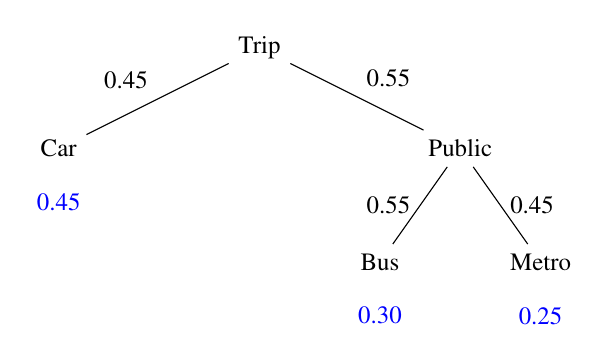
\begin{tikzpicture}[scale=0.85, every node/.style={font=\small}]
    % Root
    \node (S) at (0,0) {Trip};
    % Level 1
    \node (C) at (-3,-1.5) {Car};
    \node (P) at ( 3,-1.5) {Public};
    \draw (S) -- node[above left]  {$0.45$} (C);
    \draw (S) -- node[above right] {$0.55$} (P);
    % Level 2
    \node (Bu) at (1.8,-3.2) {Bus};
    \node (Me) at (4.2,-3.2) {Metro};
    \draw (P) -- node[left]  {$0.55$} (Bu);
    \draw (P) -- node[right] {$0.45$} (Me);
    % Joint probabilities
    \node[blue] at (1.8,-4.0) {$0.30$};
    \node[blue] at (4.2,-4.0) {$0.25$};
    \node[blue] at (-3,-2.3) {$0.45$};
\end{tikzpicture}
\end{center}

\begin{block}{Answer}
\centering \textbf{Option (a):} $0.45,\ 0.30$ and $0.25$
\end{block}
\end{frame}

%% -------------------------------------------------------
\begin{frame}{Plot}
    \begin{figure}
        \centering
        
\includegraphics[width=0.75\columnwidth]{figs/image.png}
        \caption{Probability tree diagram}
        \label{fig:placeholder}
    \end{figure}
\end{frame}

%% -------------------------------------------------------
\begin{frame}[fragile]
\frametitle{Python Code}
\begin{lstlisting}
import numpy as np
import matplotlib.pyplot as plt
import matplotlib.patches as mpatches

P_A   = 0.45
P_Ac   = 1 - P_A

P_bus_given_pub   = 0.55
P_metro_given_pub = 1 - P_bus_given_pub  

P_bus   = P_Ac * P_bus_given_pub
P_metro = P_Ac * P_metro_given_pub

labels = ['Car', 'Bus', 'Metro']
probs  = [P_A, round(P_bus, 2), round(P_metro, 2)]
colors = ['steelblue', 'darkorange', 'green']
\end{lstlisting}
\end{frame}

%% -------------------------------------------------------
\begin{frame}[fragile]
\frametitle{Python Code}
\begin{lstlisting}


plt.figure(figsize=(7, 4))
bars = plt.bar(labels, probs, color=colors, edgecolor='black', width=0.4)

for bar, val in zip(bars, probs):
    plt.text(bar.get_x() + bar.get_width()/2,
             bar.get_height() + 0.01,
             f'{val:.2f}', ha='center', fontsize=12, fontweight='bold')

plt.ylim(0, 0.6)
plt.ylabel('Probability')
plt.title('Probability of Car, Bus and Metro (CE 2008)')
plt.grid(axis='y', linestyle='--', alpha=0.6)
plt.tight_layout()
plt.savefig("image.png", dpi=300)
plt.show()
\end{lstlisting}
\end{frame}

\end{document}
